\documentclass{beamer}
\usepackage[utf8]{inputenc}
\usepackage{caption}
\usepackage{subcaption}

\title{Strategies for computing the scalar self-force on a Schwarzschild background}
\author{Steven Dorsher}
\institute{Louisiana State University}
\date{September 26, 2017}

\begin{document}
\frame{\titlepage}




\begin{frame}
  \frametitle{Gravitational Waves}
  \begin{figure}
    \includegraphics[width=3.0in]{LIGOGRtest.png}
    \caption{LIGO detection, September 14, 2015. General relativity was tested by comparing inpsiral with merger/ringdown phases.}
  \end{figure}
\end{frame}


\begin{frame}
  \frametitle{Extreme Mass Ratio Inspirals}
  \begin{figure}
    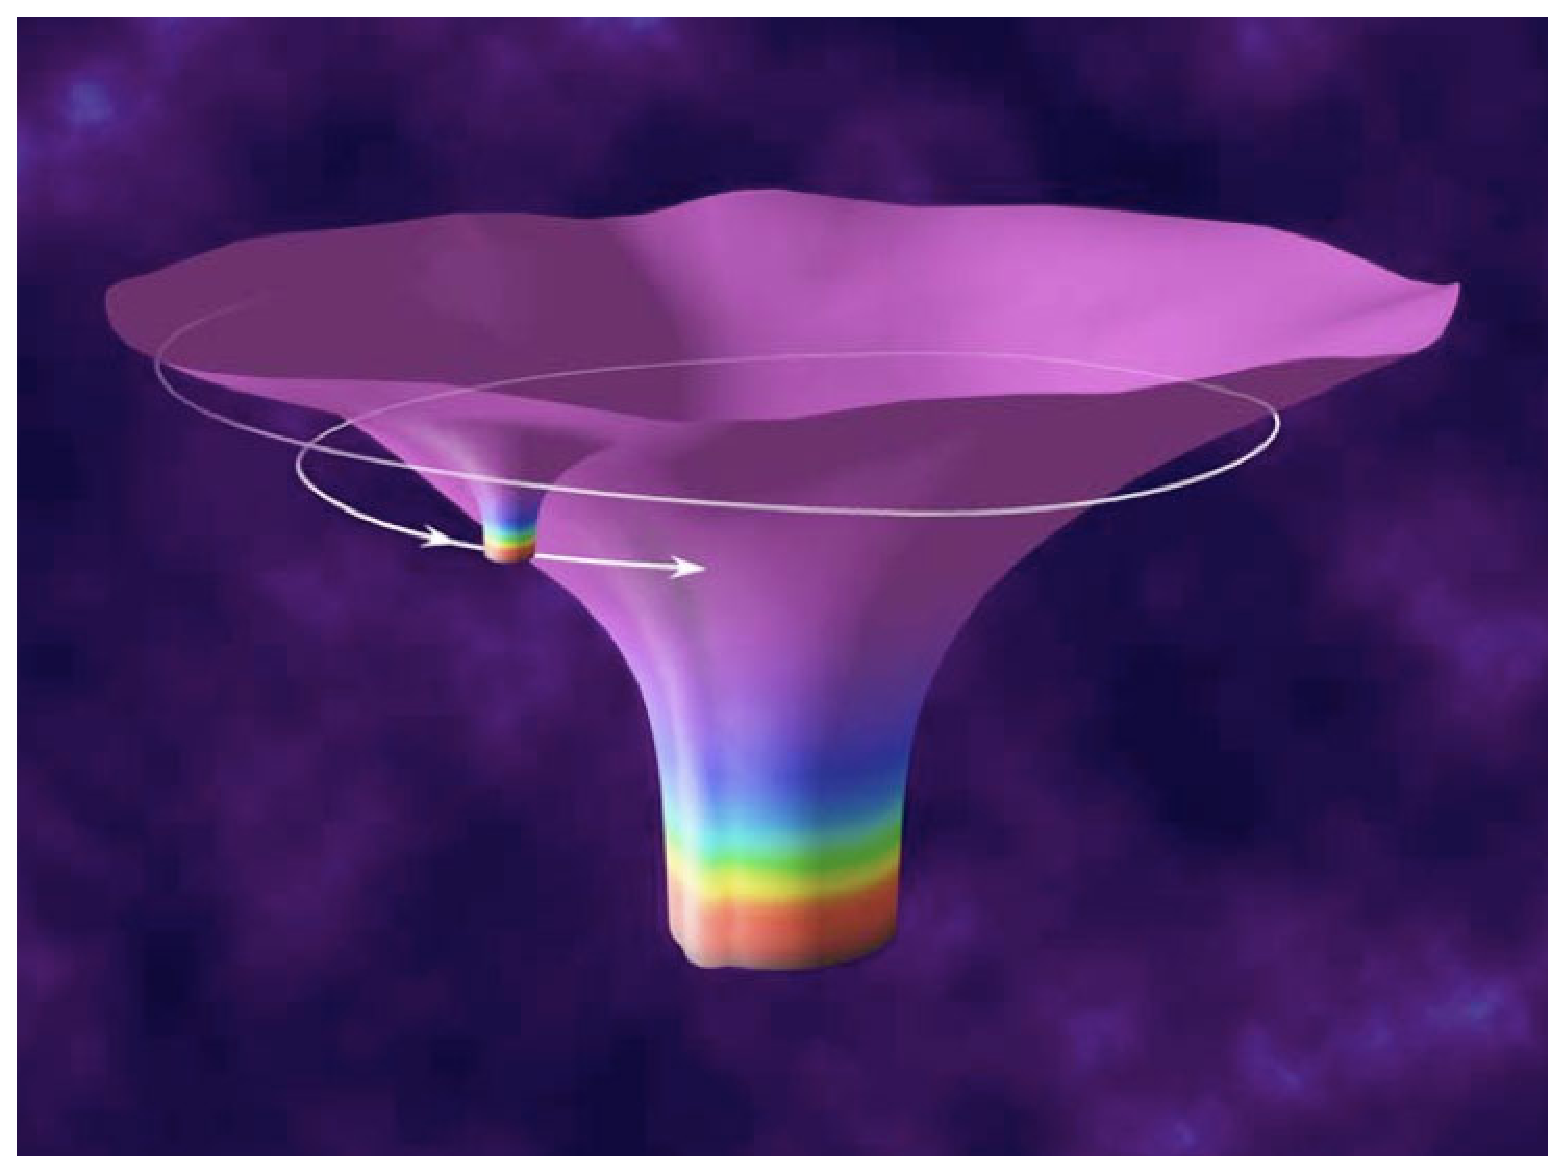
\includegraphics[width=4.0in]{EMRI}
    \citation{Extreme Mass Ratio Inspiral, $\mu=m/M\sim 10^{-4}$ to $10^{-6}$, Artist's rendition, Wikipedia}
  \end{figure}
\end{frame}

\begin{frame}
  \frametitle{Laser Interferometer Space Antenna}
  \begin{figure}
    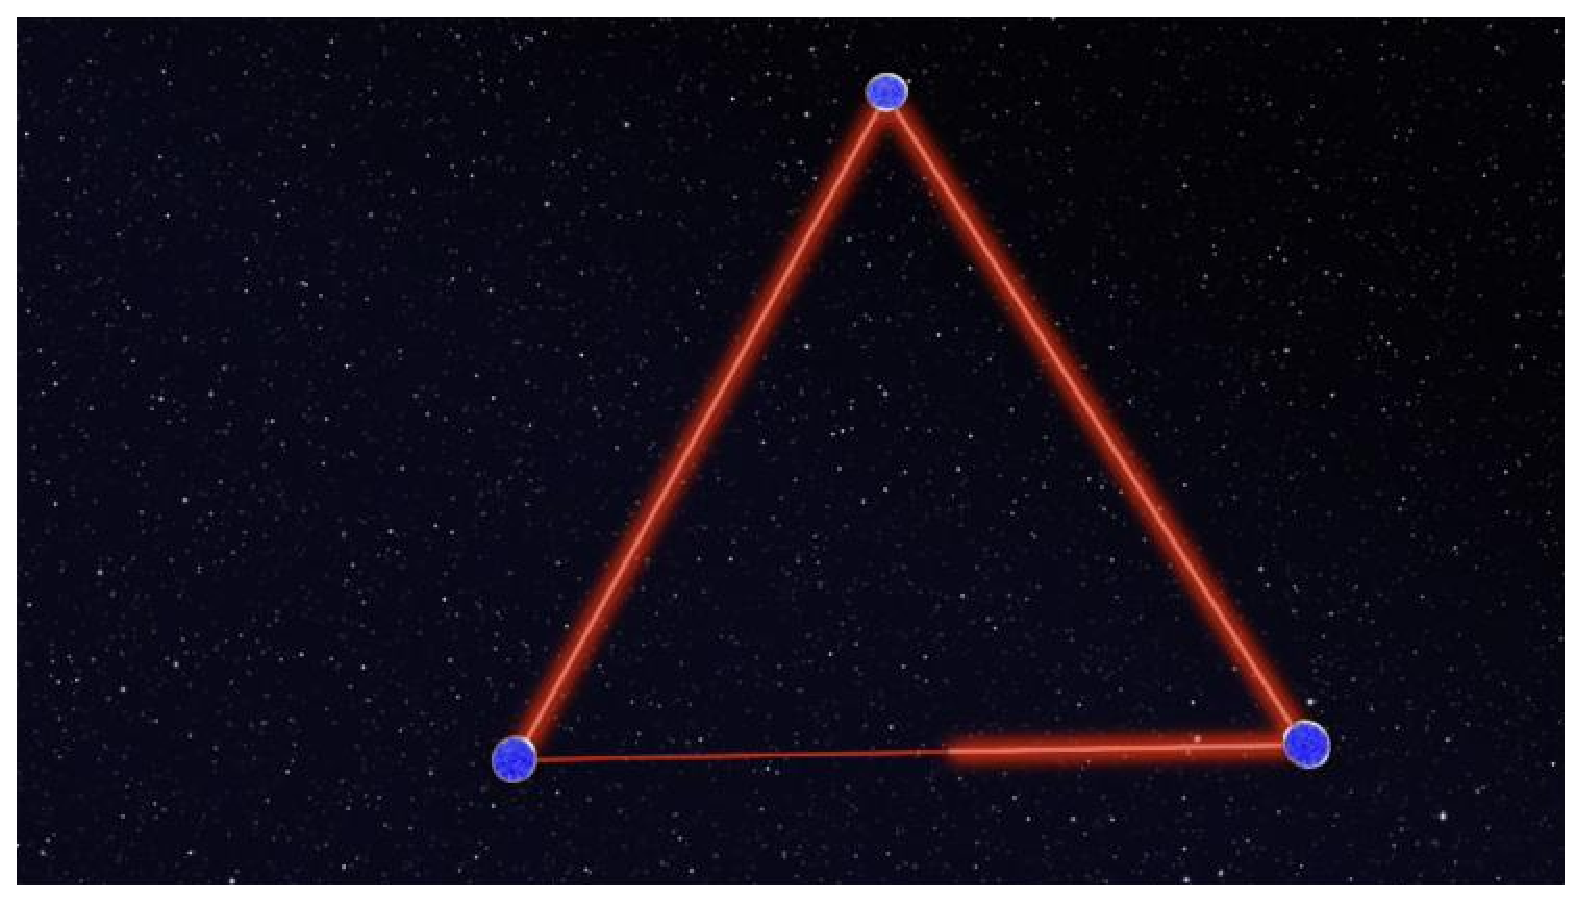
\includegraphics[width=4.0in]{eLISA}
    \caption{Laser Interferometer Space Antenna, which will operate around launches in early 2030's, ESA-NASA partnership, will detect EMRI's}
  \end{figure}
\end{frame}



\begin{frame}
  \frametitle{Toward LISA EMRI templates}
  \begin{itemize}
  \item Generating LISA EMRI templates require resolving $10^6$ orbits with precision on the order of $\delta P/P\sim 10^{-6}$ {\em Danzmann, Karsten. LISA: A proposal in response to the ESA call for L3 mission concepts (2017)}
  \item For EMRI's, the self-force approximation is used in the limit where the mass ratio is large ($10^4$ to $10^6$)
  \item Nearly equal mass numerical relativity uses spacetimes with initial conditions smoothly matched between the two blackholes, consistently evolved
  \item EMRI's have an orbital evolution timescale that scales as $M/\mu$, and a period that scales as $M$. These two widely different timescales necessitate a different numerical approach than numerical relativity.
  \item Self-force is a perturbative approximation in either the distance from the small black hole or the mass ratio. 
  \end{itemize}
\end{frame}

\begin{frame}
  \frametitle{Self-force in a classical atom}
  \begin{itemize}
  \item Consider a classical atom without quantization (not even a Bohr atom)
  \item The electron orbits the nucleus
  \item It radiates energy because it is accelerated
  \item Because it radiates energy, it becomes more tightly bound
  \item The electron spirals inward
  \item The self-force of the particle interacting with its own
      field causes this
  \end{itemize}
\end{frame}

\begin{frame}
  \frametitle{Self-force in general relativity}
  \begin{itemize}
  \item In general relativity, test particles move along geodesics
  \item A compact object is not a test particle
  \item Motion $\rightarrow$ radiation $\rightarrow$ energy and angular momentum loss $\rightarrow$ inspiral
  \item The self-force is a finite-mass particle's interaction with its own field that causes the inspiral
  \item Applies to scalar, electromagnetic, and tensor fields on a gravitational background
  \item We use perturbative expansion in terms of powers of radius from small black hole-- perturbations of the orbit
  \end{itemize}
\end{frame}

\begin{frame}
  \frametitle{Approximations and Goals}
  The long term goal for the field is to generate extremely precise EMRI gravitational wave templates for LISA.

  Approximations:
  \begin{itemize}
  \item Scalar rather than tensor waves ($\Psi$ rather than $h_{\mu\nu}$)
  \item Non-rotating black holes: Schwarzschild spacetime
  \item Self-force causes a particle to inspiral as it emits radiation
  \item We use the Detweiler-Whiting effective source as implemented by Barry Wardell
  \item In our self-consistent evolution, our self-force naturally takes into account the past history of the particle
  \item Niels Warburton assumes: the particle has been on the same geodesic for all time when he calculates the self-force
  \end{itemize}
  
  Our goal is to implement a highly accurate self-consistent evolution and do a comparison study with Niels Warburton.
  
\end{frame}


\begin{frame}
  \frametitle{Schwarzschild spacetime without a source}
  \begin{itemize}
  \item Wave equation: $\Box\Psi=\frac{1}{\sqrt{-g}}\partial_\mu\left(g^{\mu\nu}(\partial_\nu\Psi)\sqrt{-g}\right)=0$
  \item Multipole moment decomposition to account for angular dependence
  \item Quasinormal mode (QNM) ringing
    \begin{itemize}
    \item higher frequencies and faster decay for higher $l$
    \item due to interactions near peak of potential
    \end{itemize}
  \item Power law tails
    \begin{itemize}
    \item go as $t^{-(2l+3)}$
    \item follow the QNM
    \item due to scattering off spacetime far from the peak of the potential
    \end{itemize}
  \end{itemize}
\end{frame}

\begin{frame}
  \frametitle{Quasinormal modes}
  \begin{figure}
    \centering
    \begin{subfigure}{.45\textwidth}
      \centering
      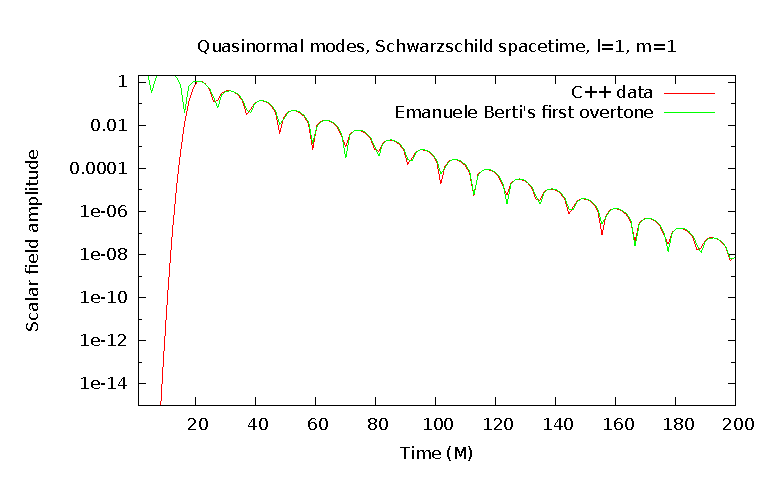
\includegraphics[width=\textwidth]{l1m1qnm}
      \caption{$l=1$}
    \end{subfigure}
    \begin{subfigure}{.45\textwidth}
      \centering
      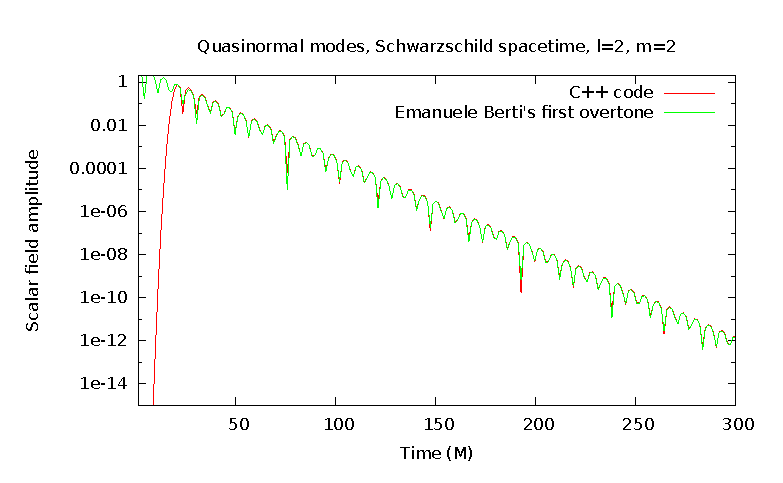
\includegraphics[width=\textwidth]{l2m2qnm}
      \caption{$l=2$}
    \end{subfigure}
  \caption{$l=2$ has a higher frequency and a faster decay rate than $l=1$}
  \end{figure}
\end{frame}

\begin{frame}
  \frametitle{Power law tails}
  \begin{figure}
    \centering
    \begin{subfigure}{.45\textwidth}
      \centering
      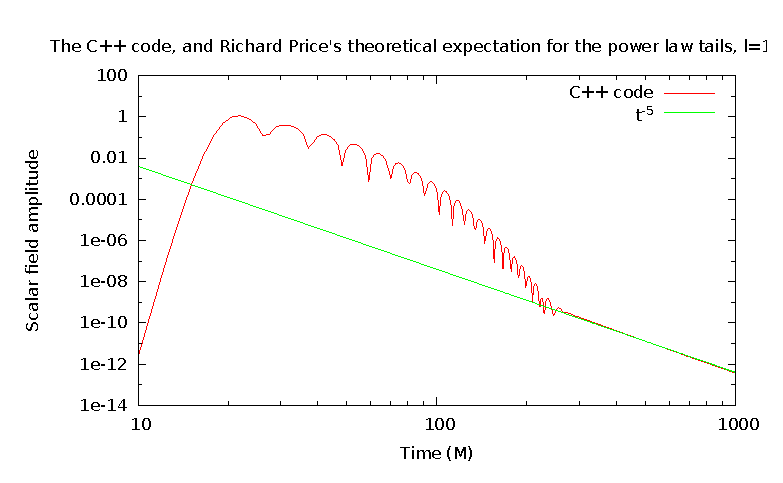
\includegraphics[width=\textwidth]{l1m1tail2}
      \caption{$l=1$}
  \end{subfigure}
    \begin{subfigure}{.45\textwidth}
      \centering
      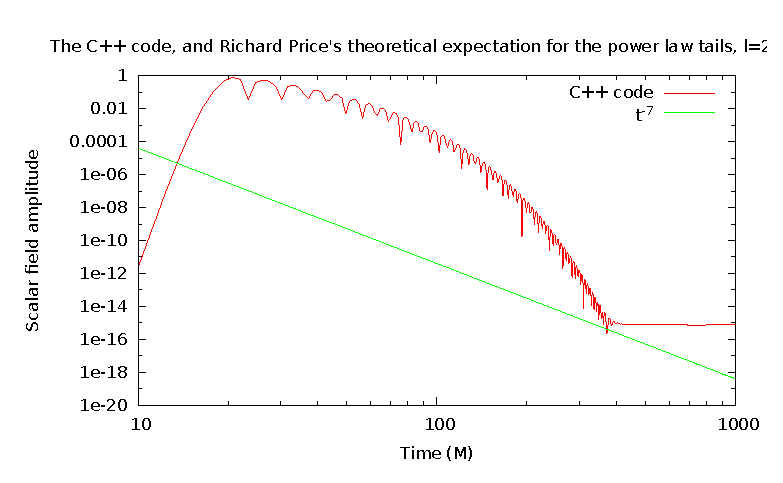
\includegraphics[width=\textwidth]{l2m2tailfail2}
      \caption{$l=2$}
    \end{subfigure}
  \caption{$l=1$ decays as $t^-{-5}$ as expected; however, $l=2$ has no power law tail due to truncation error}
  \end{figure}
\end{frame}



\begin{frame}
  \frametitle{Scalar charge on a circular orbit with an effective source}
  \begin{itemize}
  \item Self-force causes the particle to emit radiation and inspiral. An artifical force holds it on a circular orbit.
  \item Regularize field: $\Psi^R=\Psi^{ret}-\Psi^S$
  \item Detweiler-Whiting singular field: {\em Steven Detweiler, Bernard F. Whiting (2002). Phys. Rev. D 67, 024025}
  \item $\Box\Psi^R=S_{eff}=\Box\Psi^{ret}-\Box(W\tilde{\Psi}^S)=-q4\pi\int\delta_4(x,z(\tau^\prime))d\tau^\prime$
  \item Wave equation for retarded field has delta function effective source proportional to charge in the scalar case.
  \item In tensor case for gravitational field, perturbative expansion in terms of powers of radius: {\em Anna Heffernan, Adrian Ottewill, Barry Wardell (2012). Phys. Rev. D 86, 104023}
  \item I have ported this from Fortran to C++ with partially redesigned structure. I have succeeded in reproducing the results to roundoff error precision.  
  \end{itemize}
\end{frame}

\begin{frame}
  \frametitle{Circular orbit roundoff error comparison between languages}
  \begin{figure}
    \centering
    \begin{subfigure}{.45\textwidth}
      \centering
      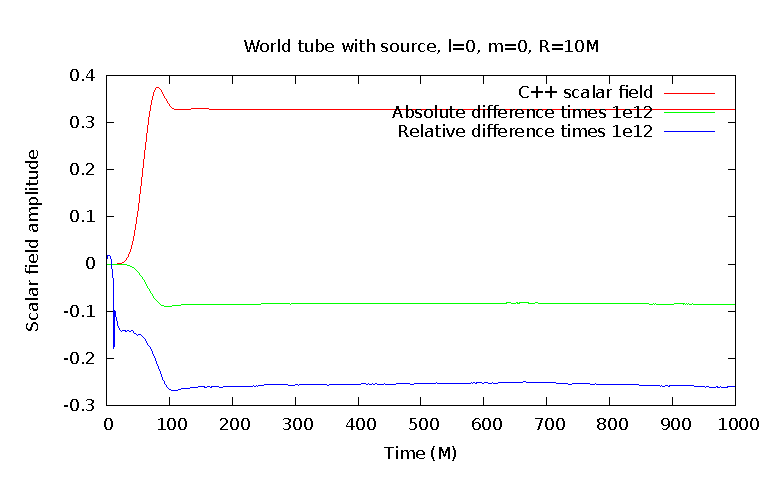
\includegraphics[width=\textwidth]{wtcircl0m0}
      \caption{l=0}
   \end{subfigure}
    \begin{subfigure}{.45\textwidth}
      \centering
      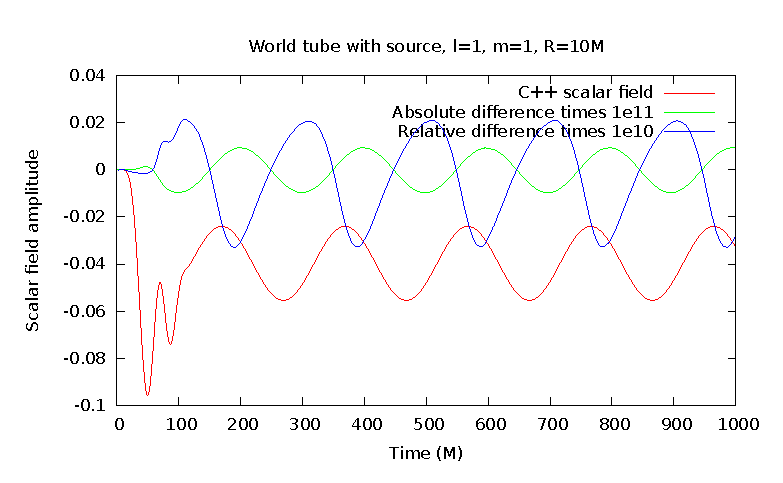
\includegraphics[width=\textwidth]{wtcircl1m1}
      \caption{l=1}
    \end{subfigure}
  \caption{Relative and absolute errors are at the roundoff level-- $10^{-10}$ to $10^{-12}$. Oscillations do not appear in the $l=0$ mode but appear with the orbital period in the $l=1$ mode.}
  \end{figure}
\end{frame}

\begin{frame}
  \frametitle{Eccentric orbits using Peter Diener's simulation}
  \begin{itemize}
  \item $\chi$, $\phi$ $\rightarrow$ precession
  \item The orbit is artifically held on a geodesic to counteract the self-force generating the scalar waves
  \item $p$, $e$ held fixed, monotonically evolving $\chi$, $\phi$
  \item $r_{periastron}=\frac{pM}{1+e}$, $r_{apastron}=\frac{pM}{1-e}$
  \item Radial self-force: $F_r=q\partial_r\Psi^R$
  \item Warburton initial conditions: particle has been on the same geodesic for all time
  \item Diener initial conditions: field starts at zero with particle at aphelion
  \end{itemize}
\end{frame}

\begin{frame}
  \frametitle{Precession of the eccentric orbit}
  \begin{figure}
    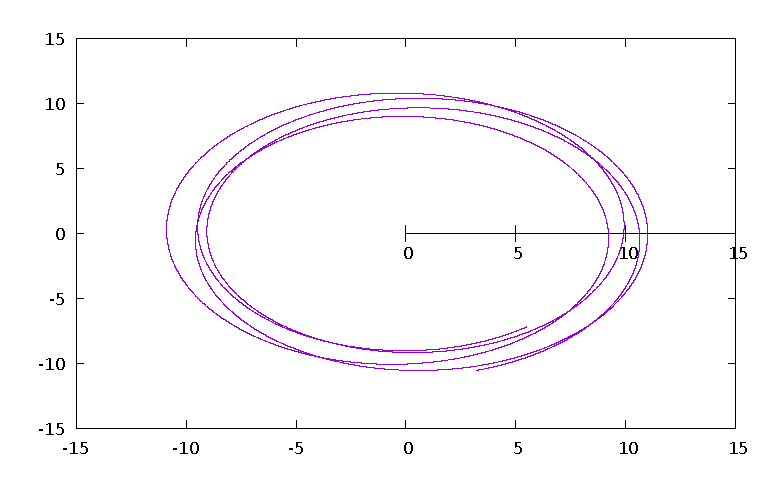
\includegraphics[width=0.9\textwidth]{orbitevolvedg44p99e01}
    \caption{Precession of the eccentric orbit. $p=9.9$, $e=0.0$.}
  \end{figure}
\end{frame}

\begin{frame}
  \frametitle{Evolution of the radial self-force for different initial conditions}
  \begin{figure}
  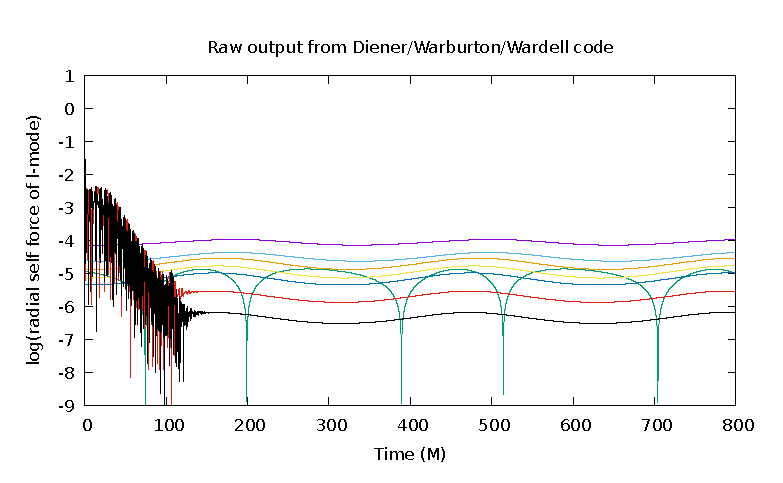
\includegraphics[width=0.9\textwidth]{rawRadialSelForceModes}
  \caption{Modes zero through seven are shown. Zero through five have smooth starts. Six and seven have transients.}
  \end{figure}
\end{frame}

\begin{frame}
  \frametitle{Addressing instabilities and error}
  \begin{itemize}
  \item I characterized the error in the eccentric evolutions due to
    \begin{itemize}
    \item Neglecting the first order Richardson extrapolation
    \item Choice of start and end modes in mode sum fit
    \item Choice of number of terms in mode sum fit
    \item Selection of weights associated with mode sum fit
    \end{itemize}
  \item Concluded the first three errors were comparable and at the $10^{-4}$ level and the fourth was negligible. This is a one order of magnitude improvement over a previous study that made use of circular orbits instead of eccentric orbits. {\em Ian Vega and Steven Detweiler (2008). Phys Rev D. 77, 084008.}
  \end{itemize}
\end{frame}

\begin{frame}
  \frametitle{The first order Richardson extrapolation}
  \begin{itemize}
  \item Discontinuous Galerkin: ODE solver with errors that scale as $h^{n+1}$
  \item Truncation error is skewed entirely to one side when measured using $L_0$ or $L_2$ error
  \item Convergent code approaches an asymptote
  \item Assume $F_r(n,l)=F_{inf}(l)+c(l)\exp(-\alpha n)$
  \item Use three different DG orders arranged in steps of four to obtain an extrapolation to $F_{inf}$ from some starting order
   \end{itemize}
\end{frame}

\begin{frame}
  \frametitle{Well-converging data}
  \begin{figure}
  \includegraphics[width=0.9\textwidth]{fittingtechniqet370l0}
  \caption{l=0 at t=370. This data converges very cleanly until it hits roundoff noise at high DG orders.}
  \end{figure}
\end{frame}
  

\begin{frame}
  \frametitle{Error due to neglecting the first order Richardson Extrapolation}
  \begin{figure}
    \includegraphics[width=0.9\textwidth]{reldiffpsirvtwfinfdgorders}
    \caption{Relative error between DG starting orders and $F_{inf}$ vs time. For DG order 36 where roundoff error sets in, the error is about $10^{-4}$.}
  \end{figure}
\end{frame}

\begin{frame}
  \frametitle{The l-mode sum and fit}
  \begin{eqnarray}
    F_r(l,t)=&\frac{A(t)}{(2l-1)(21+3)}+\frac{B(t)}{(2l-3)(2l-1)(2l+3)(2l+5)}\nonumber \\
    &+\frac{C(t)}{(2l-5)(2l-3)(2l-1)(2l+3)(2l+5)(2l+7)}+\ldots
  \end{eqnarray}

   {\em Anna Heffernan, Adrian Ottewill, Barry Wardell (2012). Phys. Rev. D 86, 104023}

  \begin{itemize}
  \item Fit from $l_{min}$ to $l_{max}$.
  \item Sum numerically from zero to $l_{max}$ then use fit coefficients to analytically sum to $l=\infty$

  \end{itemize}
\end{frame}


\begin{frame}
  \frametitle{l-mode fit}
  \begin{figure}
    \includegraphics[width=0.9\textwidth]{fiterrscalecorrect3term570l1}
    \caption{l-mode versus $F_{inf}$.}
  \end{figure}
\end{frame}

\begin{frame}
  \frametitle{Smooth evolution of total radial self-force}
  \begin{figure}
    \includegraphics[width=0.9\textwidth]{totalselfforcevt2}
     \caption{Total radial self-force including sum to $l=\infty$ over time}
  \end{figure}
\end{frame}


\begin{frame}
  \frametitle{Summary of l-mode fit results}
  \begin{itemize}
  \item The best $l_{min}=14$ and $l_{max}$=25. The relative error in these choice of values is $10^{-4}$.
  \item The relative error due to the number of terms used in the fit is $10^{-4}$.
  \item The error due to the use of weights in fitting is insignificant.
  \end{itemize}
\end{frame}

      
\begin{frame}
  \frametitle{Comparison study of self-consistent evolution to geodesic evolution}
  \begin{itemize}
  \item Self-consistent evolution accounts for the interaction of the particle with the field it has generated in the past naturally since it is evolved in the time domain
    \begin{itemize}
    \item Uses the Detweiler-Whiting singular field 
    \item The particle position evolves according to the geodesic equation with an acceleration on the right hand side
    \item The mass of the particle also evolves according to the work being done on it
    \end{itemize}
  \item Geodesic evolution uses an self-force that assumes the particle has been evolving on the same geodesic for all time
    \begin{itemize}
    \item Self-force can be efficiently calculated in the frequency domain due to periodicity
    \item Frequency domain component is good for initial conditions without transients
    \item Evolves in the time domain after generating the self-force in the frequency domain
    \item Cannot handle effects where the timescale of the orbital evolution is short compared to the period
    \end{itemize}
  \end{itemize}
\end{frame}

\begin{frame}
  \frametitle{Long term goals}
  \begin{itemize}
  \item Goal is to compare Diener's self-consistent code using Warburton's initial conditions and Wardell's effective source to Warburton's geodesic evolutions using frequency domain self force.
  \item I will run code, analyze physics, and debug, as necessary.
  \item In particular, some instabilities in the self-consistent evolutions need to be addressed before a publication will be possible. I will help look for a solution to those instabilities. 
  \item Timescale: highly variable. 2-3 years potentially?
  \end{itemize}
\end{frame}

\begin{frame}
  \frametitle{Extra slides}
\end{frame}

\begin{frame}
  \frametitle{Flat space evolution}
  \begin{figure}
    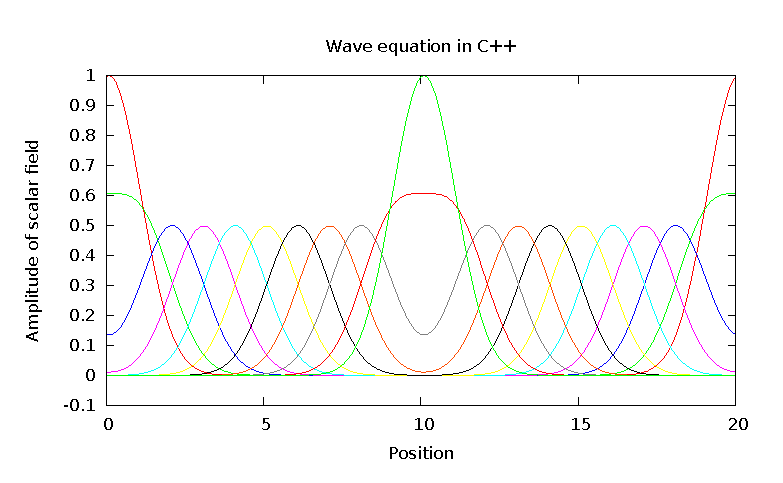
\includegraphics[width=4.0in]{gaussWave}
    \caption{Gaussian initial conditions, flat spacetime}
  \end{figure}
\end{frame}



\begin{frame}
  \frametitle{Flat spacetime error convergence}
  \begin{figure}
    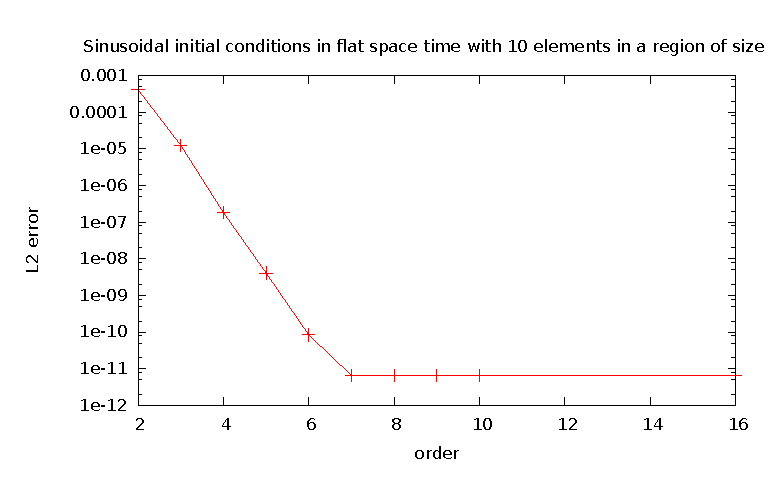
\includegraphics[width=4.0in]{sinL2WTorder}
    \caption{$L_2$ error converges exponentially until it hits roundoff noise with DG order for sinusiodal initial conditions with ten elements of size $h=0.01$.}
  \end{figure}
\end{frame}

\begin{frame}
  \frametitle{Residuals to the l-mode fit}
  \begin{figure}
    \centering
    \begin{subfigure}{.45\textwidth}
      \centering
      \includegraphics[width=\textwidth]{fitresiduals3terms570l8}
      \caption{$l_{min}=8$}
    \end{subfigure}
    \begin{subfigure}{.45\textwidth}
      \centering
      \includegraphics[width=\textwidth]{fitresidulas3terms570l14}
      \caption{$l_{min}=14$}
    \end{subfigure}
  \caption{$l_{min}=14$ is a better fit than $l_{min}=8$ both because it is less systematically biased and because it has an amplitude an order of magnitude smaller. Both fits end at $l_{max}=30$.}
  \end{figure}
\end{frame}

\begin{frame}
  \frametitle{Roundoff noise in $F_{inf}$ at high $l_{max}$}
  \begin{figure}
    \centering
    \begin{subfigure}{.45\textwidth}
      \centering
      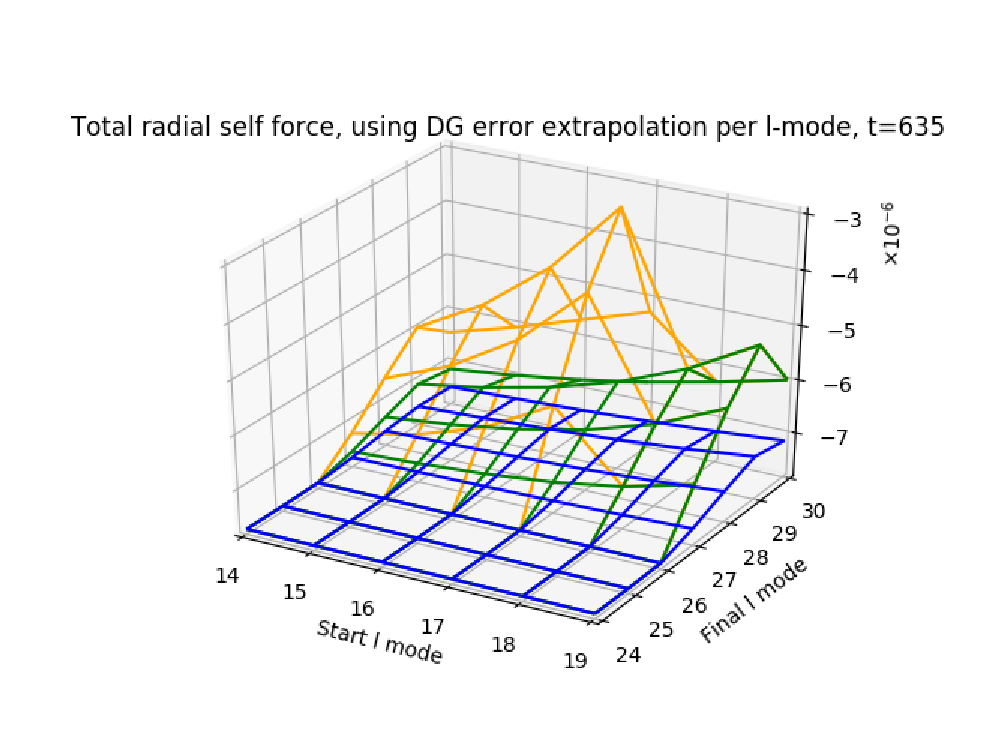
\includegraphics[width=\textwidth]{bestfinflminlmax234terms635fullrange_perihelion}
      \caption{Large range}
    \end{subfigure}
    \begin{subfigure}{.45\textwidth}
      \centering
      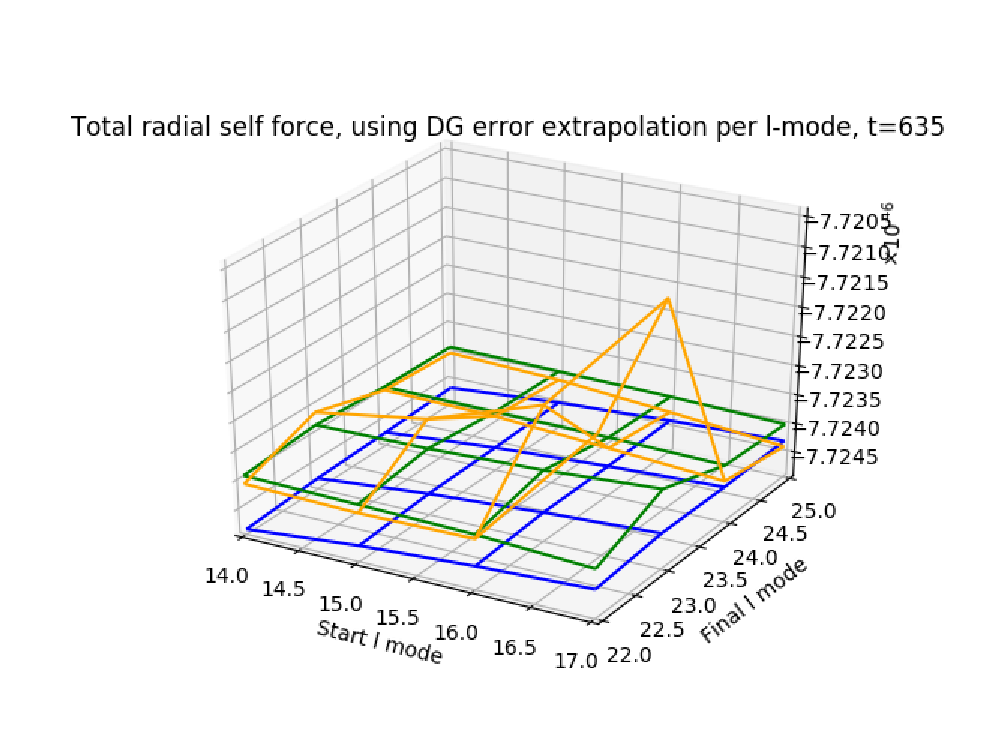
\includegraphics[width=\textwidth]{bestfinflminlmax234termst635smallrange_perihelion}
      \caption{Small range}
    \end{subfigure}
  \caption{$l_{min}=14$ and $l_{max}=25$ appear to be good start and stop values. Roundoff noise is evident at higher l.}
  \end{figure}
\end{frame}


\begin{frame}
  \frametitle{Error due to l-mode selection, number of terms}
  \begin{figure}
    \centering
    \begin{subfigure}{.45\textwidth}
      \centering
      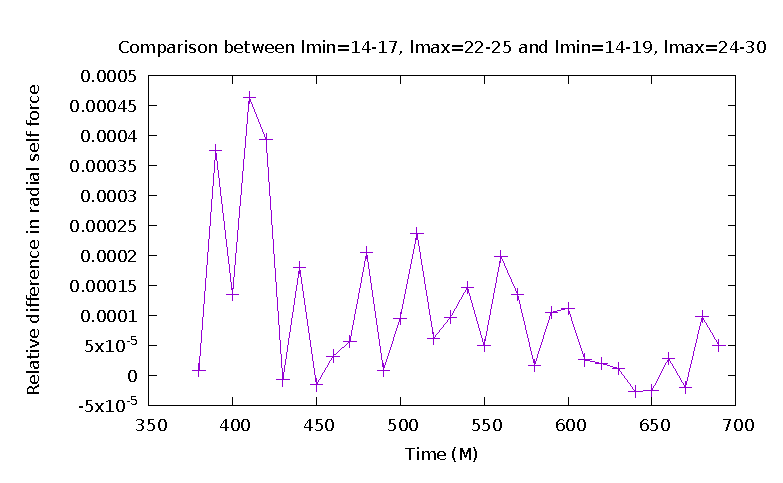
\includegraphics[width=\textwidth]{relErrBigSmallRangeOverTime}
      \caption{large versus small range}
    \end{subfigure}
    \begin{subfigure}{.45\textwidth}
      \centering
      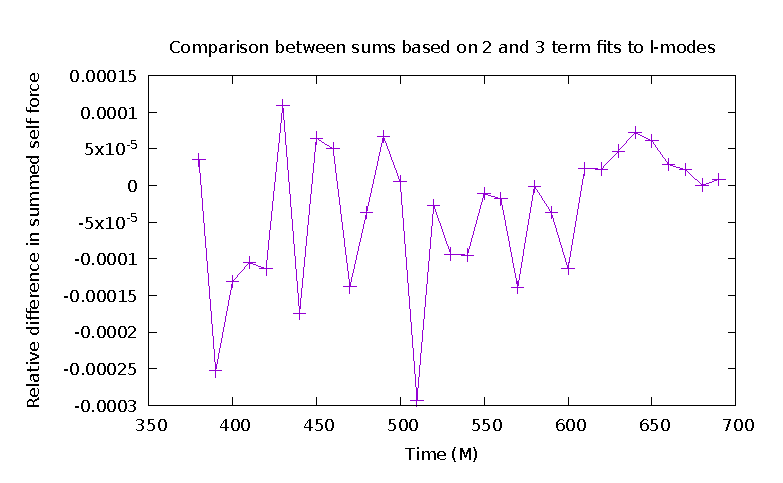
\includegraphics[width=\textwidth]{relativeError23termSelfForce}
      \caption{2 versus 3 terms}
    \end{subfigure}
  \caption{Relative errors in both of these effects appear to be at the $10^{-4}$ level.}
  \end{figure}
\end{frame}


\end{document}
